\documentclass[11pt]{article}
\usepackage[margin=0.75in]{geometry}
\usepackage{amsmath}
\usepackage{tikz}
\usepackage{enumitem}
\usepackage{color,soul}

\usepackage{multicol}


\begin{document}
\newcounter{enumCount}
\pagestyle{empty}
\subsection*{Math 141 - Homework 1 \hfill Name: \underline{\hspace*{2in}}}
\textit{For exercises 1 to 4, find the domain, range, and all zeros/intercepts, if any, of the functions.} 

\begin{multicols}{2}
\begin{enumerate}
\item $f(x) = \dfrac{x}{x^2-9}$
\item $g(x) = \sqrt{2x-1}$
\setcounter{enumCount}{\theenumi}
\end{enumerate}
\end{multicols}
\vfill


\begin{multicols}{2}
\begin{enumerate}
\setcounter{enumi}{\theenumCount}
\item $f(x) = \dfrac{1}{x^2 + 16}$
\item $h(x) = -1 + \sqrt{x+2}$
\setcounter{enumCount}{\theenumi}
\end{enumerate}
\end{multicols}
\vfill

\begin{enumerate}
\setcounter{enumi}{\theenumCount}
\item A rental car company rents cars for a flat fee of \$20 and an hourly charge of \$10.25. Therefore, the total cost $C$ to rent a car is a function of the hours $t$ the car is rented plus the flat fee.
\begin{enumerate}
\item Write the formula for the function that models this situation. \vfill
\item Find $C(48)$ and explain what it means in words. \vfill
\item Determine how long the car was rented if the bill is \$430. \vfill
\end{enumerate}


\item A certain bacterium grows in culture in a circular region. The radius of the circle, measured in centimeters, is given by $r(t)=6-[5/(t^2+1)]$, where $t$ is time measured in hours since a circle of a 1-cm radius of the bacterium was put into the culture.
\begin{enumerate}
\item Express the area of the bacteria as a function of time.\vfill
\item What is the domain of the area function?\vfill
\item Use Desmos to graph the area function.  Include a rough (hand-drawn) sketch of the graph in your solutions. Hint: Desmos always uses $x$ as the input variable, so you'll have to switch $x$ for $t$ in Desmos.  You might also need to zoom out to see what the graph really looks like. Be sure to only graph the parts of the function that correspond to realistic values of $t$.
\vfill
\vfill
\end{enumerate}

\newpage
\item A rectangle has width $x$ and diagonal length 4.  Find a formula for the area of the rectangle as a function of $x$ and determine its domain.
\begin{flushright}
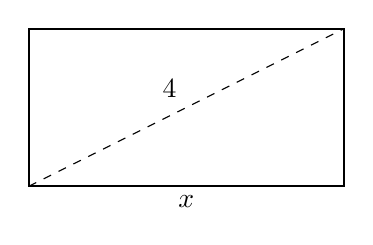
\begin{tikzpicture}
\draw[thick] (0,0) rectangle (4,2);
\draw[dashed] (0,0) -- (2,1) node[above left] {4} -- (4,2);
\draw (2,0) node[below] {$x$};
\end{tikzpicture}
\end{flushright}

\item Imagine a spherical planet made of rock that is covered in a uniform layer of ice.  Suppose that the rocky part of the planet has radius $3.0 \times 10^6$ meters, and the ice layer is $x$ meters deep. Find a formula for the volume of the ice as a function of $x$. Recall that the volume of a sphere is $(4/3)\pi r^3$. \vfill 

\item Find an equation for the line that passes through $(-1,4)$ and $(3,-1)$ \vfill
\item Find an equation for the line that passes through $(-3,2)$ with slope $\tfrac{2}{3}$. \vfill
\item Find an equation for the line with $x$-intercept 6 and $y$-intercept $-9$. \vfill

\item Find the slope and $y$-intercept of the line $2x + 3y = 6$. \vfill

\item A condominium in an upscale part of the city was purchased for \$432,000. In 30 years it is worth \$129,000. Find the rate of depreciation.
\setcounter{enumCount}{\theenumi}
\end{enumerate}
\vfill


\end{document}
